\documentclass[border=4pt]{standalone}
\usepackage[T1]{fontenc}
\usepackage{lmodern}
\usepackage{amsmath}
\usepackage{pgfplots}
\pgfplotsset{compat=1.18}
\usepgfplotslibrary{groupplots,fillbetween}
\usetikzlibrary{calc,arrows.meta}
% one colour per kind of method, the same in every figure (Okabe-Ito)
\definecolor{neur}{HTML}{D55E00}   % neurons chosen by attribution
\definecolor{dirc}{HTML}{009E73}   % directions from the weird-vs-normal contrast
\definecolor{read}{HTML}{0072B2}   % readout methods and interventions chosen from readouts
\definecolor{pers}{HTML}{CC79A7}   % Assistant Axis / persona
\definecolor{ctrl}{HTML}{8C8C8C}   % random controls
\definecolor{meas}{HTML}{E69F00}   % measured outcome
\definecolor{ink}{HTML}{222222}
\pgfplotsset{
  every axis/.append style={clip=false, font=\small, axis line style={black!55}, tick style={black!55}, tick align=outside,
    label style={font=\small}, tick label style={font=\footnotesize}, title style={font=\small, align=center}},
  grid style={black!9, line width=0.4pt},
  every axis legend/.append style={font=\footnotesize, draw=none, fill=none},
  ci/.style={/pgfplots/error bars/x dir=both, /pgfplots/error bars/x explicit, /pgfplots/error bars/error bar style={line width=0.8pt}, /pgfplots/error bars/error mark=none},
  yci/.style={/pgfplots/error bars/y dir=both, /pgfplots/error bars/y explicit, /pgfplots/error bars/error bar style={line width=0.8pt}, /pgfplots/error bars/error mark=none},
}

\begin{document}
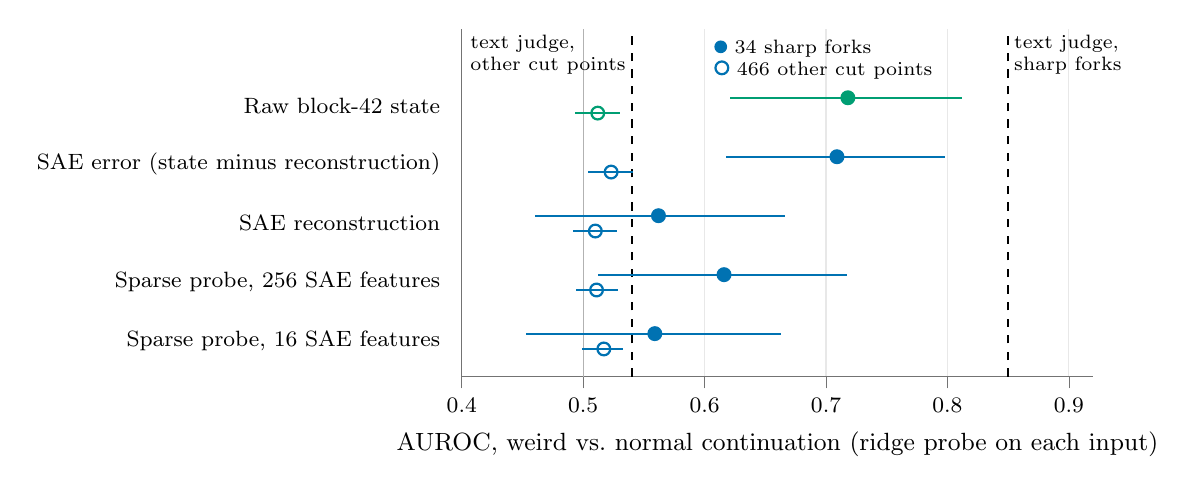
\begin{tikzpicture}
\begin{axis}[width=9.6cm, height=6.0cm, ymin=-4.60, ymax=1.3, ytick={0.00,-1.00,-2.00,-3.00,-4.00}, yticklabels={{Raw block-42 state},{SAE error (state minus reconstruction)},{SAE reconstruction},{Sparse probe, 256 SAE features},{Sparse probe, 16 SAE features}}, y tick label style={font=\footnotesize}, major y tick style={draw=none}, axis y line*=left, axis x line*=bottom, xmajorgrids, xmin=0.4, xmax=0.92, xtick={0.4,0.5,0.6,0.7,0.8,0.9}, xticklabel style={/pgf/number format/.cd, fixed, precision=1}, xlabel={AUROC, weird vs.\ normal continuation (ridge probe on each input)}]
\draw[black!30, line width=0.5pt] (axis cs:0.5,-4.60) -- (axis cs:0.5,1.3);
\draw[black, dashed, line width=0.8pt] (axis cs:0.850,-4.60) -- (axis cs:0.850,1.3);
\node[font=\scriptsize, anchor=north west, align=left, inner sep=2pt] at (axis cs:0.850,1.3) {text judge,\\sharp forks};
\draw[black, dashed, line width=0.8pt] (axis cs:0.540,-4.60) -- (axis cs:0.540,1.3);
\node[font=\scriptsize, anchor=north east, align=left, inner sep=2pt] at (axis cs:0.540,1.3) {text judge,\\other cut points};
\addplot[only marks, mark=*, mark size=2.3pt, dirc, line width=0.8pt, ci] coordinates {(0.718,0.13) += (0.094,0) -= (0.097,0)};
\addplot[only marks, mark=o, mark size=2.3pt, dirc, line width=0.8pt, fill=white, ci] coordinates {(0.512,-0.13) += (0.018,0) -= (0.019,0)};
\addplot[only marks, mark=*, mark size=2.3pt, read, line width=0.8pt, ci] coordinates {(0.709,-0.87) += (0.089,0) -= (0.091,0)};
\addplot[only marks, mark=o, mark size=2.3pt, read, line width=0.8pt, fill=white, ci] coordinates {(0.523,-1.13) += (0.018,0) -= (0.019,0)};
\addplot[only marks, mark=*, mark size=2.3pt, read, line width=0.8pt, ci] coordinates {(0.562,-1.87) += (0.104,0) -= (0.102,0)};
\addplot[only marks, mark=o, mark size=2.3pt, read, line width=0.8pt, fill=white, ci] coordinates {(0.510,-2.13) += (0.018,0) -= (0.018,0)};
\addplot[only marks, mark=*, mark size=2.3pt, read, line width=0.8pt, ci] coordinates {(0.616,-2.87) += (0.101,0) -= (0.104,0)};
\addplot[only marks, mark=o, mark size=2.3pt, read, line width=0.8pt, fill=white, ci] coordinates {(0.511,-3.13) += (0.018,0) -= (0.017,0)};
\addplot[only marks, mark=*, mark size=2.3pt, read, line width=0.8pt, ci] coordinates {(0.559,-3.87) += (0.104,0) -= (0.106,0)};
\addplot[only marks, mark=o, mark size=2.3pt, read, line width=0.8pt, fill=white, ci] coordinates {(0.517,-4.13) += (0.016,0) -= (0.018,0)};
\node[font=\scriptsize, anchor=north west, align=left] at (axis cs:0.6,1.28) {\tikz\fill[read] (0,0) circle (2.3pt); 34 sharp forks\\ \tikz\draw[read, line width=0.8pt] (0,0) circle (2.3pt); 466 other cut points};
\end{axis}
\end{tikzpicture}
\end{document}
